\section{Компьютерные эксперименты}\label{sec_exp}
\subsection{График рассеяния зависимой пеменной и регрессоров}
Чтобы зрительно представлять, как выбросы влияют на функцию регрессии, был построен график рассеяния зависимой переменной и регрессоров: $(y_i^{\widetilde{\varepsilon}}, x_i)$.

Бралась выборка объема $N = 1000$. Доля выбросов $\widetilde{\varepsilon}$ равнялась $0.08$. 
Параметры регрессии выбирались $(90, 4)^T$. 
Регрессоры $x_i$ выбирались из равномерного распределения $\sim U(-5,5)$. 
Ошибки экспериментов подчинялись нормальному закону распределения с параметрами $(0, 16)$. Выбросы подчинялись нормальному распрелению с параметрами $(100, 100)$. 

\begin{figure}[h!]
    \centering
    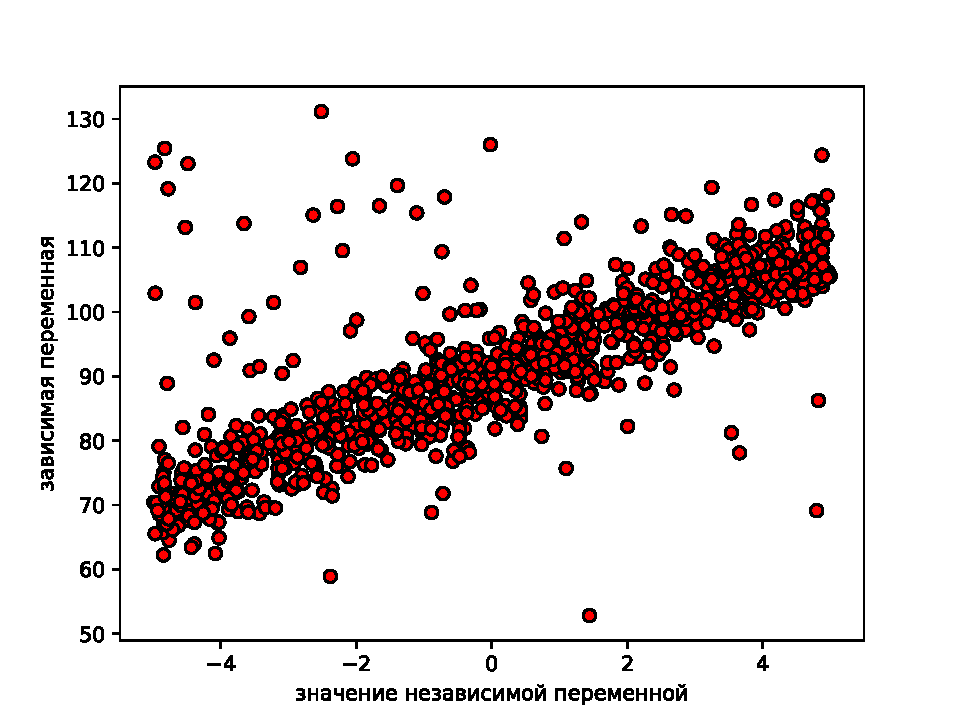
\includegraphics[width=100mm]{../images/scatter.pdf}
    \caption{График рассеяния $(y_i^{\widetilde{\varepsilon}}, x_i)$\label{overflow}}
    \label{pic_scatter}
\end{figure}

На рисунке \ref{pic_scatter} видно, что часть аномальных наблюдений сильно отстоит от генеральной совокупности наблюдений и поэтому вносят сильное искажение в результирующие группированые наблюдения, но при этом, по всей видимости, может быть выявлена при переклассификации.
Остальная часть аномальных наблюдений ''смешивается'' с генеральной совокупностью и поэтому плохо выявляется при переклассификации.

\newpage


\subsection{Вариации оценок МНК и М-оценок в случае линейной регрессии с выбросами}\label{ss_1}
Далее было проведено сравнение, как ведет себя классический метод и робастный метод в случае возникновения аномальных наблюдений в выборке.

На следующих двух графиках изображено изменение вариаций М-оценок и МНК оценок при увеличении объема выборки.

\begin{figure}[h!]
    \centering
    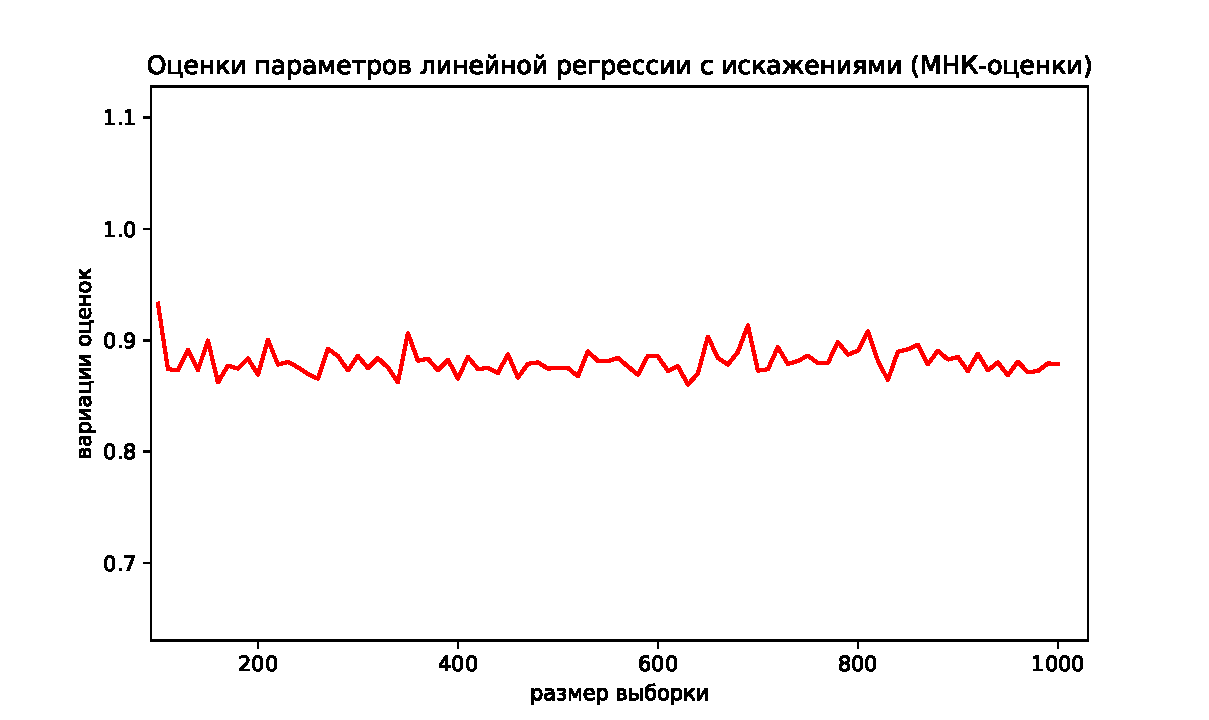
\includegraphics[width=100mm]{../images/OLS.pdf}
    \caption{Вариации оценок МНК в зависимости от объема выборки при постоянной доле выбросов\label{overflow}}
    \label{pic_ols}
\end{figure}

\begin{figure}[h!]
    \centering
    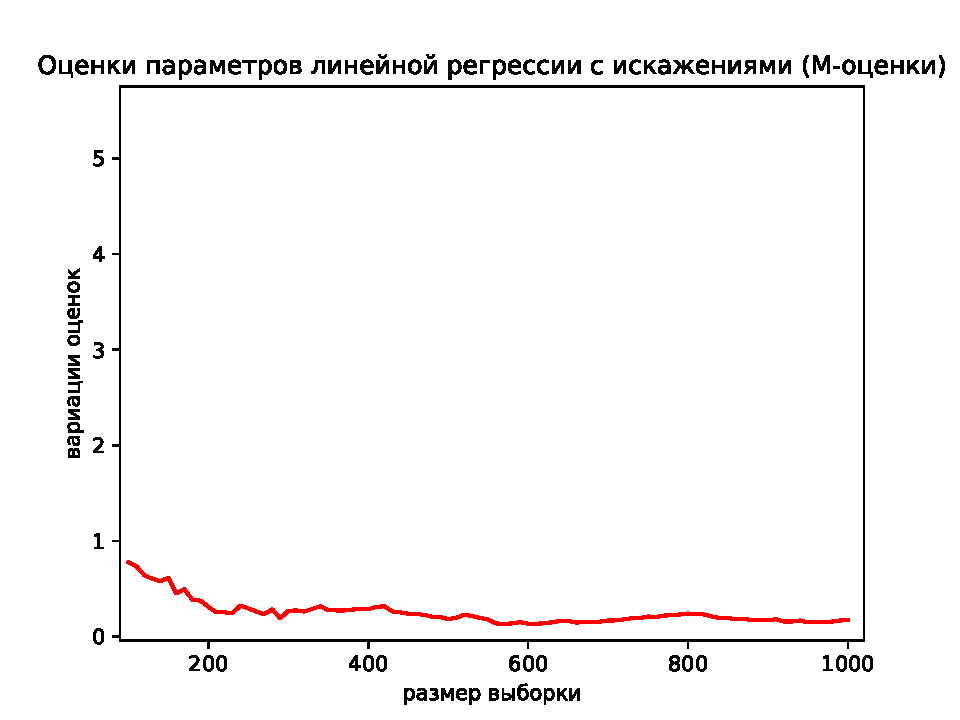
\includegraphics[width=100mm]{../images/RLM(1).pdf}
    \caption{Вариации оценок М-оценок в зависимости от объема выборки при постоянной доле выбросов\label{overflow}}
\end{figure}

Объем выборки изменялся от $N=100$ до $N=1000$. 
Доля выбросов $\widetilde{\varepsilon}$ равнялась $0.08$. 
Параметры регрессии выбирались $(90, 4)^T$. 
Регрессоры $x_i$ выбирались из равномерного распределения $\sim U(-5,5)$. 
Ошибки экспериментов подчинялись нормальному закону распределения с параметрами $(0, 16)$. Выбросы подчинялись нормальному распрелению с параметрами $(100, 100)$. 

На графиках видно, что робастные М-оценки в отличие от оценок МНК сходятся с увеличением объема выборки. 
Рисунок \ref{pic_ols} показывает, почему важна задача построения робастных методов оценивания параметров регрессии: классический метод (оценки МНК) не сходится при увеличении объема выборки.

\subsection{Вариации оценок без переклассификации}
Далее был проведен похожий эксперимент на эксперимент в пункте \ref{ss_1}, но кроме аномальных наблюдений присутствовало группирование выборки. Использовались построенные ОМП-оценки, но не применялась переклассификация выборки. 

Объем выборки $N$ изменялся от $N_1=140$ до $N_2=300$, при этом выборка дополнялась, а не генерировалась новая. Использовалась модель линейной регрессии. Доля выбросов была постоянна и равнялась $\widetilde{\varepsilon}=0.08$. 
Регрессоры $x_i$ были из равномерного распределения $U(-5,5)$.  Параметры регрессии были постоянными и равнялись $\beta=(90,4)^T$. Ошибки эспериментов $\varepsilon_i\sim \mathcal{N}(0,16)$.
На графики изображено изменение вариаций оценок при увеличении объема выборки.
\begin{figure}[hb]
    \centering
    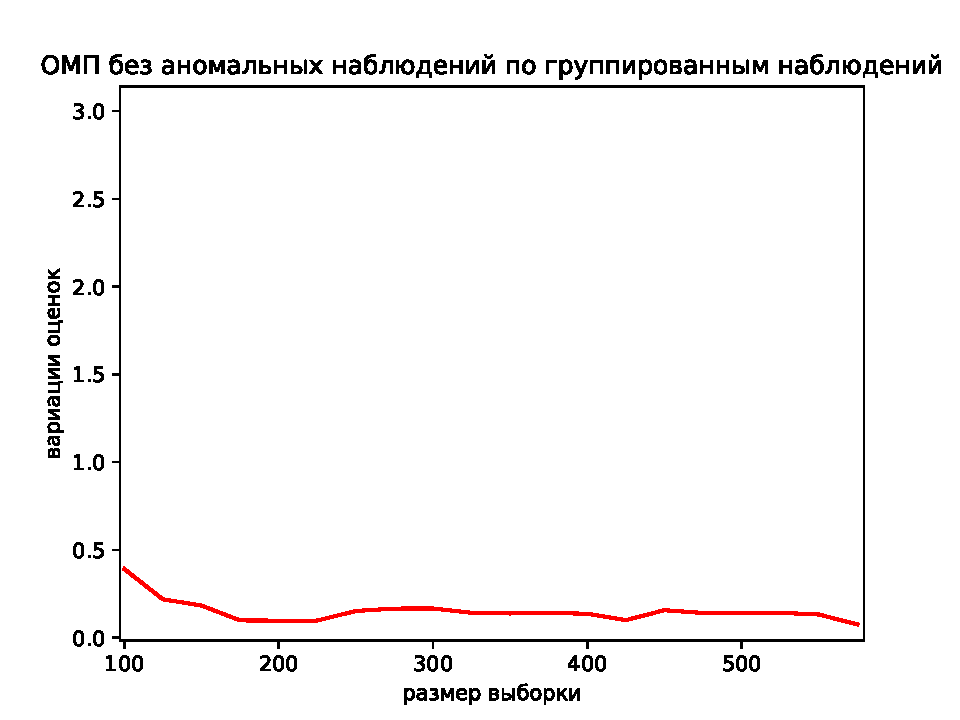
\includegraphics[width=100mm]{../images/MLE_no_outliers(2).pdf}
    \caption{Зависимость вариаций от размера выборки\label{overflow}}
    \label{pic6}
\end{figure}

С увеличением объема выборки построенные ОМП-оценки сходятся, но так как в выборке присутствуют аномальные наблюдения, скорость сходимости метода невелика и дисперсия вариаций оценок очень большая. 

\subsection{Графики рассеяния оценок в случае использования метода K-ближайших соседей для переклассификации}
Далее к выборке с аномальными наблюдениями с группированием применялась переклассификации, а после этого применялись построенные ОМП-оценки.

На следующих двух графиках (рис. \ref{pic4} - рис. \ref{pic5}) изображена диаграмма рассеяния, если для переклассификации выборки выбран метод $K$-ближайших соседей.

Для построения рисунка \ref{pic4} генерировались выборки объема $N = 1000$. Доля выбросов $\widetilde{\varepsilon}$ равнялась $0.08$. 
Параметры регрессии выбирались $(90, 4)^T$. 
Регрессоры $x_i$ выбирались из равномерного распределения $\sim U(-5,5)$. 
Ошибки экспериментов подчинялись нормальному закону распределения с параметрами $(0, 16)$. Выбросы подчинялись нормальному распрелению с параметрами $(100, 100)$. 

\begin{figure}[h]
    \centering
    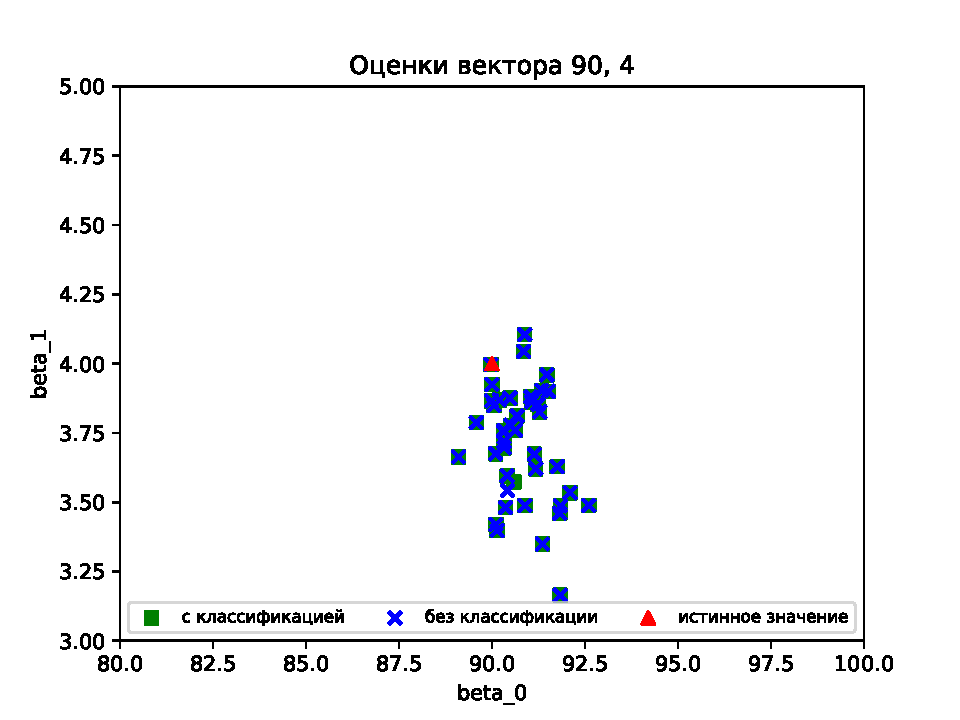
\includegraphics[width=110mm]{../images/plot_90_4_with-without_(3).pdf}
    \caption{График рассеяния $(\hat{\beta}_0,\hat{\beta}_1)$\label{overflow}}
    \label{pic4}
\end{figure}

Для построения рисунка \ref{pic5} генерировались выборки объема $N = 1000$. Доля выбросов $\widetilde{\varepsilon}$ равнялась $0.08$. 
Параметры регрессии выбирались $(90, 4)^T$. 
Регрессоры $x_i$ выбирались из равномерного распределения $\sim U(-5,5)$. 
Ошибки экспериментов подчинялись нормальному закону распределения с параметрами $(0, 16)$. Выбросы подчинялись нормальному распрелению с параметрами $(100, 100)$. 
\newpage

\begin{figure}[h]
    \centering
    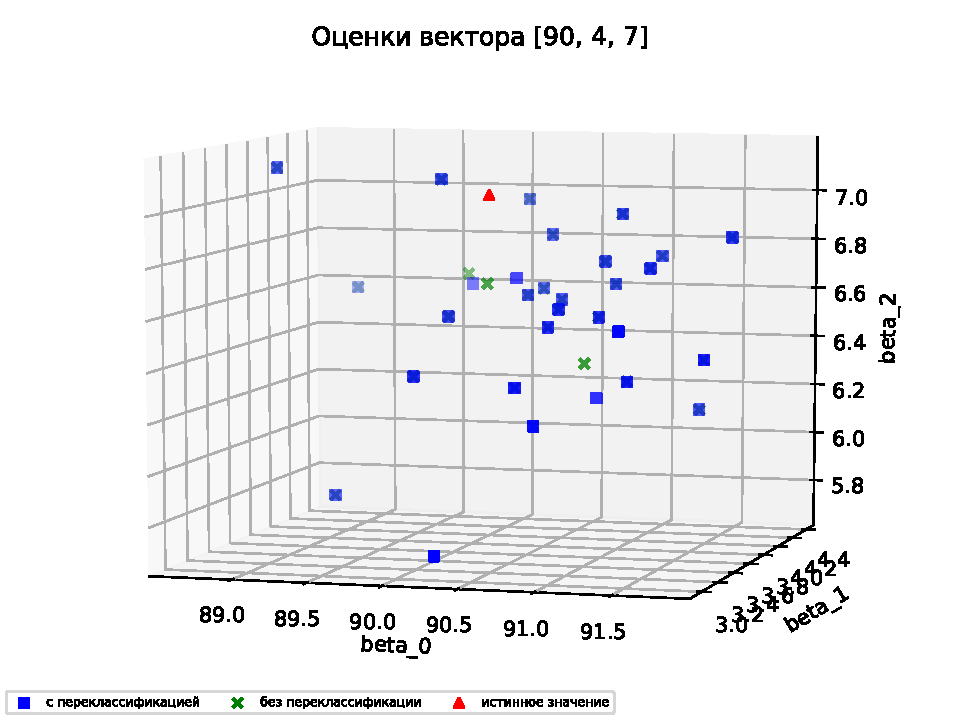
\includegraphics[width=100mm]{../images/plot_90_4_7_(4).pdf}
    \caption{График рассеяния $(\hat{\beta}_0,\hat{\beta}_1, \hat{\beta}_2)$\label{overflow}}
    \label{pic5}
\end{figure}

На полученных рисунках видно, что оценки параметров получаются близкими при разных выборках.

\subsection{Сравнение оценок при переклассификации методом K-ближайших соседей с оценками без переклассификации}
Были проведены эксперименты для сравнения эмпирической вариации оценок максимального правдоподобия, когда использовалась переклассификация методом K-ближайших соседей и когда не использовалась. При этом на каждой итерации выборка увеличивалась. 

Объем выборки $N$ изменялся от $N_1=100$ до $N_2=400$, при этом выборка дополнялась, а не генерировалась новая. Использовалась модель линейной регрессии. Доля выбросов была постоянна и равнялась $\widetilde{\varepsilon}=0.08$. Параметры регрессии были постоянными и равнялись $\beta=(90,4)^T$. 
Регрессоры $x_i$ были из равномерного распределения $U(-5,5)$, ошибки эспериментов $\varepsilon_i\sim \mathcal{N}(0,16)$. В методе, где использовалась переклассификация, величина $K$ выбиралась: $K=10$.
\newpage
\vspace{3cm}
\begin{center}
    \captionof{table}{Параметры модели и оценок экспериментов}\label{tab1}
    \begin{tabular}{|p{5cm}|p{5cm}|}
        \hline
        \multicolumn{2}{|c|}{Параметры программы} \\
        \hline
        Переменная&значение\\
        \hline
        Размер выборки $N$& от 100 до 400\\
        \hline
        Доля выбросов $\widetilde{\varepsilon}$& 0.08\\
        \hline
        Параметры регрессии $\beta$& $(90,4)$\\
        \hline
        Регрессоры $x_i$ & $\sim U(-5,5)$\\
        \hline
        $\varepsilon_i$&$\sim \mathcal{N}(0,16)$\\
        \hline
        $\eta_i$&$\sim \mathcal{N}(100,100)$\\
        \hline
        В методе, с переклассификацией величина $K$& 10\\
        \hline
    \end{tabular},
\end{center}

\begin{figure}[ht!]
    \centering
    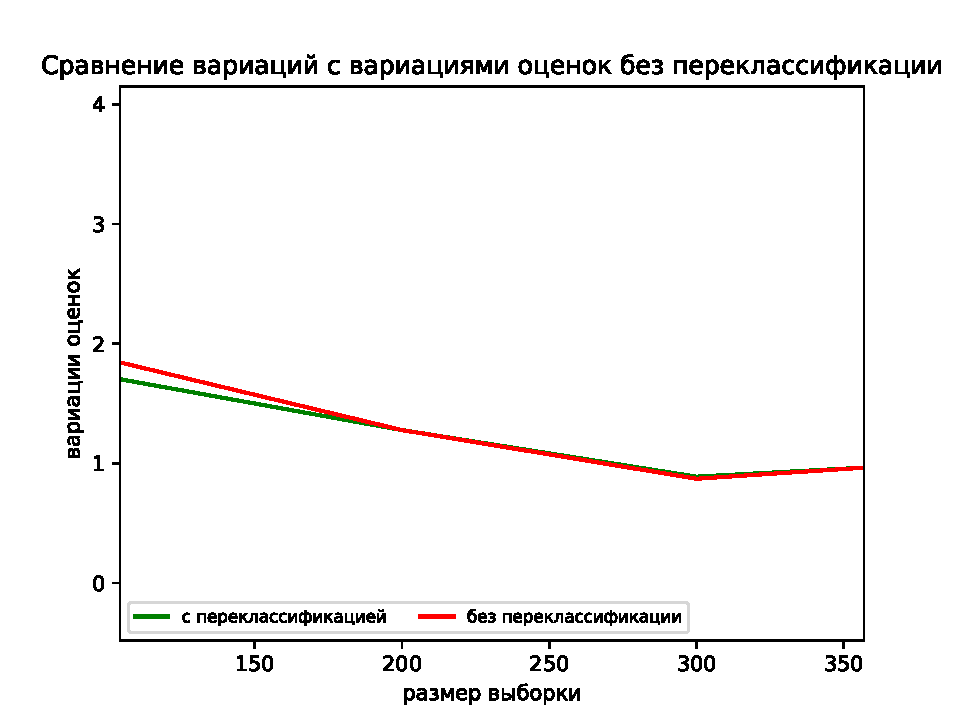
\includegraphics[width=100mm]{../images/on_off_recl.pdf}
    \caption{Сравнение вариаций оценок максимального правдоподобия когда используется и не используется переклассификация\label{overflow}}
    \label{pic2}
\end{figure}

% \subsection{Параметры модели и оценок}
% В ходе экспериментов использовались следующие параметры модели:
% \begin{center}
%     \begin{tabular}{|p{5cm}|p{5cm}|}
%         \hline
%         \multicolumn{2}{|c|}{Параметры программы} \\
%         \hline
%         Переменная&значение\\
%         \hline
%         Размер выборки $N$& 1000\\
%         \hline
%         Доля выбросов $\widetilde{\varepsilon}$& 0.08\\
%         \hline
%         Параметры регрессии $\beta$& $(90,4)$\\
%         \hline
%         Регрессоры $x_i$ & $\sim U(-5,5)$\\
%         \hline
%         $\varepsilon_i$&$\sim N(0,16)$\\
%         \hline
%         $\eta_i$&$\sim N(100,100)$\\
%         \hline
%         Величина $K$ из пункта 2.3 курсового проекта &$10$\\
%         \hline
%     \end{tabular},
% \end{center}
% \newpage

\subsection{Сравнительный анализ оценок максимального правдоподобия с альтернативной} \label{ss_4_6}
\subsubsection{Эксперимент с изменением объема выборки}
В следующем эксперименте был произведен сравнительный анализ вариаций ОМП-оценок с МНК оценками в зависимости от объема выборки.

Объем выборки $N$ изменялся от $N_1=100$ до $N_2=500$, при этом выборка дополнялась, а не генерировалась новая. Использовалась модель линейной регрессии. Доля выбросов была постоянна и равнялась $\widetilde{\varepsilon}=0.08$. Параметры регрессии были постоянными и равнялись $\beta=(90,4)^T$. 
Регрессоры $x_i$ были из равномерного распределения $U(-5,5)$, ошибки эспериментов $\varepsilon_i\sim \mathcal{N}(0,16)$. Для переклассификации использовался метод $K$-ближайших соседей.

\begin{center}
    \captionof{table}{Параметры модели и оценок}\label{tab1}
    \begin{tabular}{|p{5cm}|p{5cm}|}
        \hline
        \multicolumn{2}{|c|}{Параметры программы} \\
        \hline
        Переменная&значение\\
        \hline
        Размер выборки $N$& от 100 до 500\\
        \hline
        Доля выбросов $\widetilde{\varepsilon}$& 0.08\\
        \hline
        Параметры регрессии $\beta$& $(90,4)$\\
        \hline
        Регрессоры $x_i$ & $\sim U(-5,5)$\\
        \hline
        $\varepsilon_i$&$\sim \mathcal{N}(0,16)$\\
        \hline
        $\eta_i$&$\sim \mathcal{N}(100,100)$\\
        \hline
        Величина $K$  &$10$\\
        \hline
    \end{tabular},
\end{center}
\begin{figure}[h!]
    \centering
    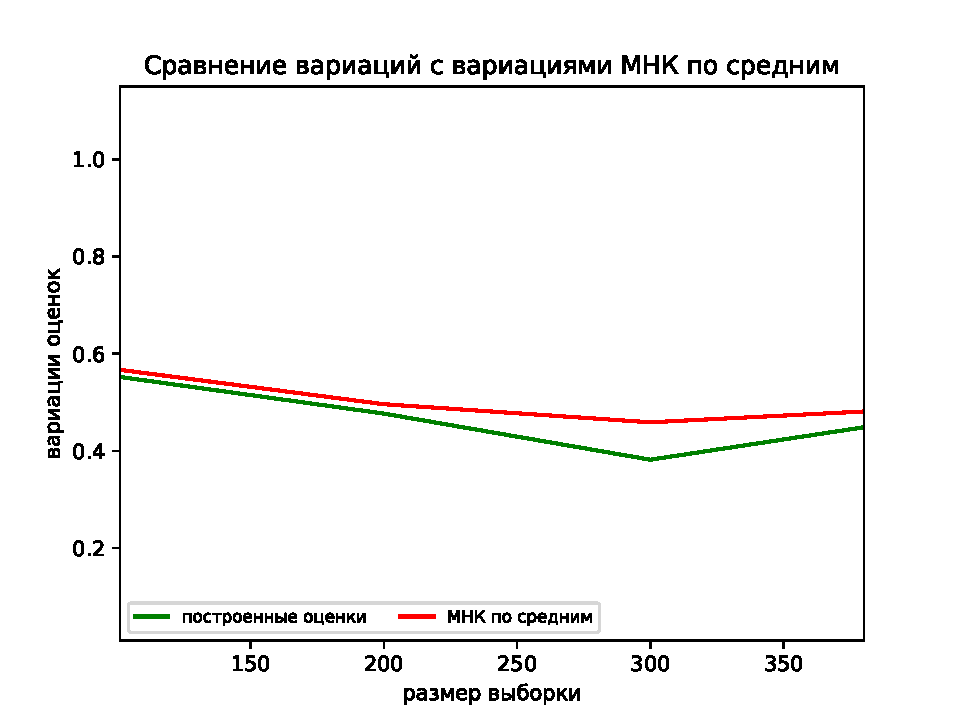
\includegraphics[width=100mm]{../images/OLS_GEM.pdf}
    \caption{Сравнение вариаций оценок\label{overflow}}
    \label{pic0}
\end{figure}
При сравнении графиков вариаций (рис.\ref{pic0}) можно сделать вывод, что ОМП дают лучший результат, 

\subsubsection{Эксперимент с полиномиальной регрессией}
Был проведен эксперимент с полиномиальной регрессией. Использовались те же параметры модели (таблица \ref{tab1}), объем выборки $N$ изменялся от 100 до 1000:
\newpage
\begin{figure}[h!]
    \centering
    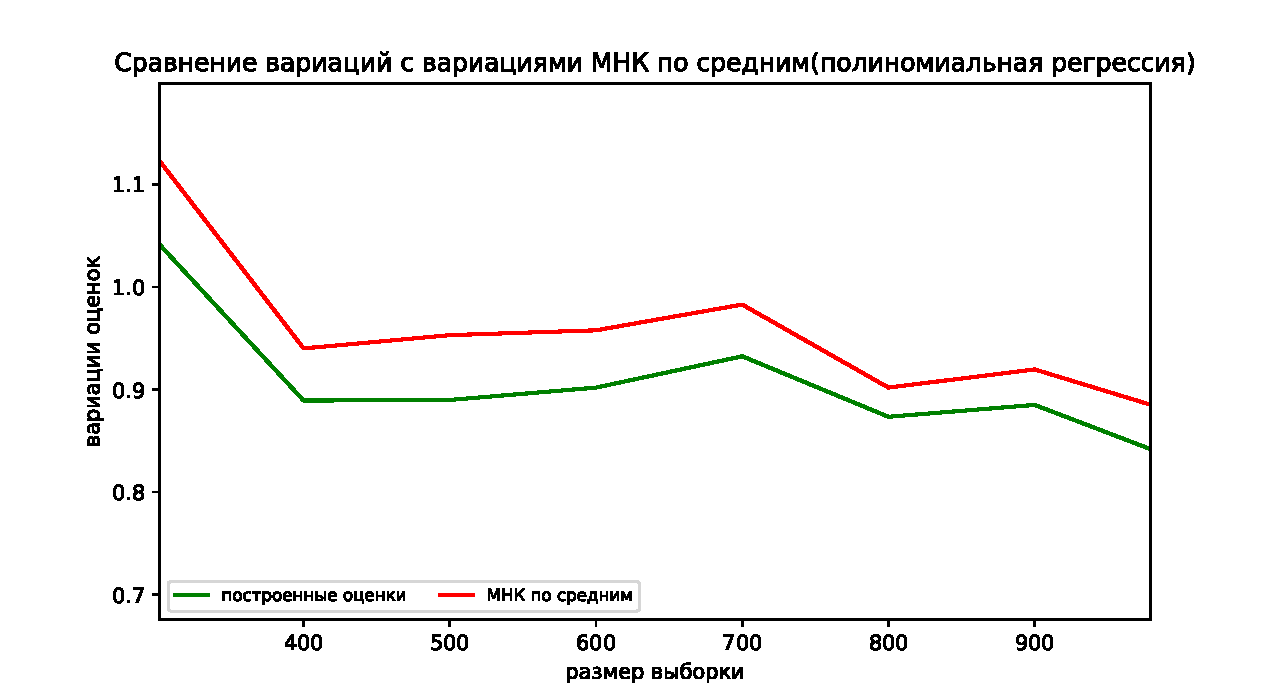
\includegraphics[width=150mm]{../images/polynomial.pdf}
    \caption{Вариации оценок в случае полиномиальной регрессии\label{overflow}}
    \label{pic3}
\end{figure}

Оба метода имели схожее поведение при изменении объема выборки, но построенные оценки максимального правдоподобия стабильно показывали лучший результат.

\subsection{Эксперименты с изменением уровня переклассификации выборки для метода $K$-ближайших соседей}\label{ss3_3_1}
В ходе дипломной работы были построены эксперименты с изменением величины K для метода $K$-ближайших соседей, используемого в переклассификации.  

Объем выборки $N$ был постоянным: $N=500$. Использовалась модель линейной регрессии. Доля выбросов была постоянна и равнялась $\widetilde{\varepsilon}=0.08$. Параметры регрессии были постоянными и равнялись $\beta=(90,4)^T$. 
Регрессоры $x_i$ были из равномерного распределения $U(-5,5)$, ошибки эспериментов $\varepsilon_i\sim \mathcal{N}(0,16)$. Величина $K$ менялась от $10$ до $40$.
\newpage
\begin{center}
    \captionof{table}{Параметры модели и оценок экспериментов с переклассификацией выборки}\label{tab1}
    \begin{tabular}{|p{5cm}|p{5cm}|}
        \hline
        \multicolumn{2}{|c|}{Параметры программы} \\
        \hline
        Переменная&значение\\
        \hline
        Размер выборки $N$& 500\\
        \hline
        Доля выбросов $\widetilde{\varepsilon}$& 0.08\\
        \hline
        Параметры регрессии $\beta$& $(90,4)$\\
        \hline
        Регрессоры $x_i$ & $\sim U(-5,5)$\\
        \hline
        $\varepsilon_i$&$\sim \mathcal{N}(0,16)$\\
        \hline
        $\eta_i$&$\sim \mathcal{N}(100,100)$\\
        \hline
        Величина $K$  &от $10$ до $40$\\
        \hline
    \end{tabular},
\end{center}

\begin{figure}[h!]
    \centering
    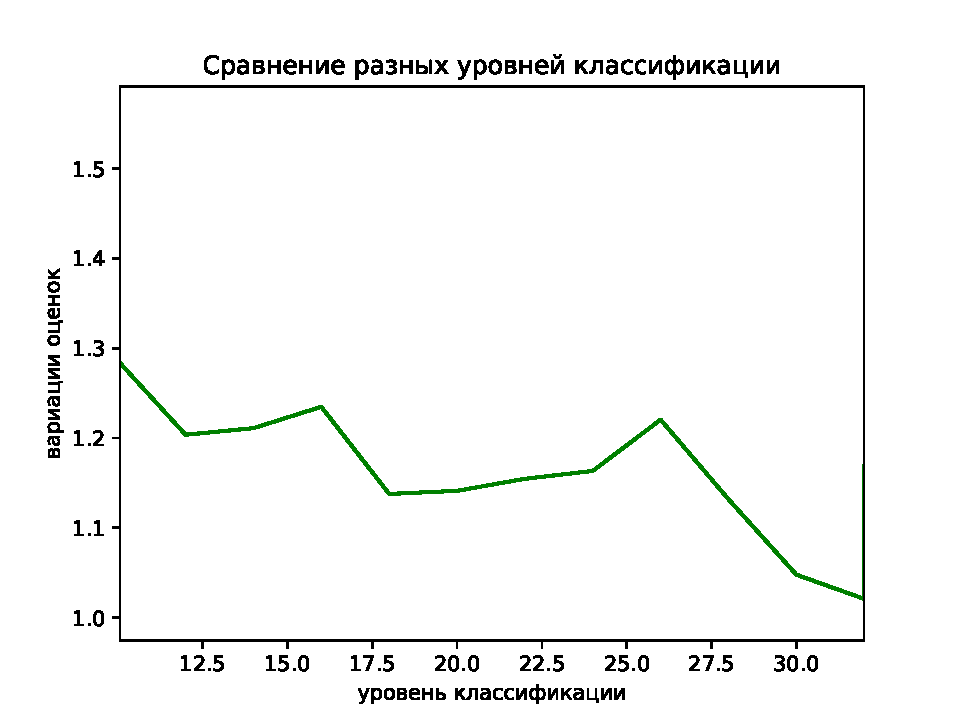
\includegraphics[width=100mm]{../images/different_recl_level.pdf}
    \caption{Зависимость вариаций от $K$ -- числа соседей, используемого в переклассификации выборки\label{overflow}}
    \label{pic1}
\end{figure}

В результате получилось, что при увеличении константы K точность оценки параметров растёт. 

\subsection{Эксперименты с изменением K для Local outlier factor, используемого в переклассификации}\label{ss3_3_2}
В ходе экспериментов была построена таблица, где выписаны $K$ для выборки определенного объема с определенной длиной интервала, то есть такую величину $K$, при которой количество неверных классов после переклассификации не более чем такое количество до переклассификации (значения получены опытным путём).
Доля выбросов была постоянна и равнялась $\widetilde{\varepsilon}=0.08$. Параметры регрессии были постоянными и равнялись $\beta=(90,4)^T$. 
Регрессоры $x_i$ были из равномерного распределения $U(-5,5)$, ошибки эспериментов $\varepsilon_i\sim \mathcal{N}(0,16)$.

\begin{center}
    \captionof{table}{Подходящие значения $K$ для выборки определенного объема с определенной длиной интервала}\label{tab2}
    \begin{tabular}{|p{5cm}|p{5cm}|p{5cm}|}
        \hline
        Объем выборки&длина интервала& величина $K$\\
        \hline
        1000 & 2.0 & 2\\
        1000 & 3.0 & 4\\
        1000 & 4.0 & 4\\

        3000 & 1.0 & 2\\
        3000 & 1.5 & 2\\
        3000 & 1.75 & 3\\
        3000 & 2.0 & 5\\
        3000 & 4.0 & 7\\

        10000 & 1.0 & 2\\
        10000 & 1.5 & 3\\
        10000 & 2.0 & 6\\
        10000 & 4.0 & 8\\
        \hline
    \end{tabular},
\end{center}
Далее приведен пример получаемых в ходе экспериментов значений.
было смоделировано $10^5$ наблюдений. Процент аномальных наблюдений: $8\%$. Константа $K$ равнялась 3.
\begin{Verbatim}[fontsize=\scriptsize]
    modulated with outlier count: 8047
    fit: classified
    wrong outliers: 7987
    fit: reclassificator scored 0.925034 on learning set:
    fit: reclassified 10
    
    fit: classified
    
    Classes differ with/without outliers when without reclassification: 7604
    Classes differ with/without outliers when with reclassification: 7582
\end{Verbatim}

Число 8047 - количество выбросов в выборке.

Число 7987 - количество ошибочно определенных выбросов (то есть ошибки рода: отнести выбросы к истинным значениям или истинные значения к выбросам). Хотим, чтобы было по крайней мере меньше предыдущего значения.

Число 7604 - количество неверных значений изначально, то есть неверных значений, полученных извне (это число может быть меньше 8047 так как при достаточно широких классах выбросы могли попасть в нужный класс)

Число 7582 - результат переклассификации, который мы хотим получить меньше предыдущего числа (7604). Чем меньше - тем лучше.


\subsection{Влияние переклассификации методом LOF на вариации оценок} \label{ss_4_9}
На следующем графике показано изменение вариаций ОМП и ОМП с переклассификацией методом, где используется локальный уровень выброса и случайный лес.
Объем выборки изменялся от $N=500$ до $N=800$. 
Доля выбросов $\widetilde{\varepsilon}$ равнялась $0.08$. 
Параметры регрессии выбирались $(90, 4)^T$. 
Регрессоры $x_i$ выбирались из равномерного распределения $\sim U(-5,5)$. 
Ошибки экспериментов подчинялись нормальному закону распределения с параметрами $(0, 16)$. Выбросы подчинялись нормальному распрелению с параметрами $(100, 100)$. 

\begin{figure}[hb]
    \centering
    \includegraphics[width=100mm]{../images/LOF_without(1).pdf}
    \caption{Зависимость вариаций от размера выборки\label{overflow}}
\end{figure}

На данном графике видно, что возможна сходимость оценок, а также в целом видно, что переклассификация очень хорошо влияет на точность результатов.

\newpage

\newpage
